\documentclass[11pt,a4paper]{article}

\usepackage[a4paper,
            top=25mm, bottom=25mm,
            left=25mm, right=25mm,
            headheight=15pt]{geometry}

\usepackage[utf8]{inputenc}
\usepackage{amsmath,amssymb}
\usepackage{graphicx}
\usepackage{booktabs}
\usepackage{hyperref}
\usepackage[dvipsnames]{xcolor}
\usepackage{tikz}
\usetikzlibrary{arrows.meta,decorations.pathreplacing,patterns,calc,matrix}
\usepackage{pgfplots}
\pgfplotsset{compat=1.18}
\usepackage[numbers,sort&compress]{natbib}
\usepackage{fancyhdr}
\usepackage{microtype}
\usepackage{siunitx}
\usepackage{listings}
\usepackage{caption}

\pagestyle{fancy}
\fancyhf{}
\lhead{\small SAMBP TR-15/2026 --- 87L Voltage-Based Pi-Section Correction}
\rhead{\small PhD Thesis Supporting Report}
\cfoot{\thepage}

\hypersetup{colorlinks=true, linkcolor=blue!70!black, citecolor=OliveGreen,
            urlcolor=blue!70!black}

\newcommand{\sambp}{\textsc{sambp}}
\newcommand{\Idiff}{I_{\mathrm{diff}}}
\newcommand{\Ifund}{I_{\mathrm{fund}}}
\newcommand{\fint}{f_{\mathrm{int}}}
\newcommand{\alphaThresh}{\alpha_{\mathrm{thresh}}}
\newcommand{\alphafifty}{\alpha_{50}}
\newcommand{\kappan}{\kappa_n}
\newcommand{\BC}{B_C}
\newcommand{\pu}{\,\text{pu}}
\newcommand{\IC}{I_{C}}

\lstset{basicstyle=\ttfamily\small,
        keywordstyle=\color{blue!70!black},
        commentstyle=\color{gray},
        frame=single, breaklines=true}

%=======================================================================
\begin{document}
%=======================================================================

\begin{center}
  {\LARGE\bfseries SAMBP Technical Report TR-15/2026}\\[6pt]
  {\large 87L Line Differential: Voltage-Based Pi-Section Correction\\
          and Final Threshold Reduction to 0.08\,pu}\\[4pt]
  \today
\end{center}

\vspace{4pt}
\noindent\rule{\linewidth}{0.6pt}

\begin{abstract}
SAMBP TR-13 improved 87L high-impedance fault (HIF) sensitivity by replacing
the fixed-amplitude charging compensation with a pre-fault blind correction,
achieving $\alphafifty(\mathrm{ag}) = 0.05$ and lowering the detection
threshold to $I_{\mathrm{thresh}} = 0.12\pu$.  TR-13 identified that further
threshold reduction required voltage measurements at both line terminals
(TR-13 Future Work~1).  This report implements Mode~1: the pi-section
charging current is predicted sample-by-sample from both-end voltage
measurements using a Hilbert-transform-based estimator, with no pre-fault
window requirement.  The residual noise floor is limited only by the
voltage-transformer (PT) accuracy class ($\sigma_{\mathrm{PT}} = 0.001\pu$),
enabling the detection threshold to be safely reduced to $0.08\pu$ with a
tighter sensitivity range ($k_{\mathrm{max}} = 2.0$).  A 200-trial Monte
Carlo sweep gives $\alphafifty(\mathrm{ag}) = 0.03$ and
$\alphafifty(\mathrm{3ph}) = 0.02$, representing a 40\% reduction from the
TR-13 result and a cumulative 57\% reduction from the TR-11 baseline.  The
voltage-based correction requires no changes to the LM estimator or
confidence gate and is backward-compatible with the existing SAMBP 87L
pipeline.
\end{abstract}

\noindent\rule{\linewidth}{0.6pt}

\tableofcontents
\vspace{6pt}

%=======================================================================
\section{Background and Motivation}
\label{sec:background}
%=======================================================================

\subsection{Sensitivity improvement chain: TR-11 to TR-15}

The 87L line differential protection against high-impedance faults has been
progressively improved across four SAMBP reports:

\begin{enumerate}
  \item \textbf{TR-11}~\cite{SAMBP_TR11}: identified the fundamental
        sensitivity floor caused by the Stage-2 confidence gate suppressing
        correct trips when $\Ifund$ falls below the 0.20\pu threshold at low
        fault currents.  Established $\alphafifty$ as the sensitivity metric.

  \item \textbf{TR-12}~\cite{SAMBP_TR12}: magnitude override bypasses the
        confidence-gate veto when $\Ifund \geq 0.30\pu$, improving
        $\alphafifty(\mathrm{ag})$ from 0.10 to 0.07.

  \item \textbf{TR-13}~\cite{SAMBP_TR13}: pre-fault blind correction reduces
        the charging residual from 0.018\pu to 0.001\pu, enabling
        $I_{\mathrm{thresh}} = 0.12\pu$ and $\alphafifty(\mathrm{ag}) = 0.05$.

  \item \textbf{TR-15} (this report): voltage-based correction (Mode~1)
        removes the pre-fault window requirement and enables
        $I_{\mathrm{thresh}} = 0.08\pu$, achieving $\alphafifty(\mathrm{ag}) = 0.03$.
\end{enumerate}

\subsection{Residual floor of the TR-13 pre-fault method}

The pre-fault blind correction (TR-13) achieves its residual improvement by
fitting the single-frequency model
\begin{equation}
  i_{\rm diff,pre}(t) \approx A_C \cos(\omega t) + B_C \sin(\omega t)
  \label{eq:prefault_fit}
\end{equation}
to the one-cycle pre-fault window using linear least-squares.  The residual
of this fit, 0.001\pu RMS, is limited by two factors:

\begin{enumerate}
  \item \textbf{Load-flow variation}: the actual terminal voltages deviate
        from the nominal by $\pm5$--10\% in magnitude and $\pm3^\circ$ in
        phase, introducing an amplitude uncertainty in the charging current
        estimate.  A 20-ms pre-fault window averages over one full cycle of
        load variation, reducing this to $\approx 0.001\pu$.

  \item \textbf{Window requirement}: the pre-fault correction requires at
        least 20\,ms of clean pre-fault data before it can be applied.  At
        fault inception within an already-disturbed system (e.g.\ during a
        busbar transfer as described in TR-14), this window may not be
        available, forcing fallback to the nominal model (residual
        0.018\pu, threshold reverts to 0.20\pu).
\end{enumerate}

The voltage-based method addresses both limitations simultaneously.

%=======================================================================
\section{Voltage-Based Correction (Mode 1)}
\label{sec:mode1}
%=======================================================================

\subsection{Pi-section charging current}

For a lumped pi-section transmission line, the differential charging current
measured at the relay is:
\begin{equation}
  i_{C,\rm diff}(t)
  = \frac{\BC}{2} \frac{\mathrm{d}v_S}{\mathrm{d}t}\bigg/\omega
  + \frac{\BC}{2} \frac{\mathrm{d}v_R}{\mathrm{d}t}\bigg/\omega
  = \BC \cdot \mathrm{Im}\!\left\{\mathcal{H}\!\left[\frac{v_S + v_R}{2}\right]\right\}
  \label{eq:ic_hilbert}
\end{equation}
where $\BC = \omega C_{\rm total}$ is the line susceptance, $v_S(t)$ and
$v_R(t)$ are the local and remote terminal voltages, $\mathcal{H}[\cdot]$
denotes the Hilbert transform, and $\mathrm{Im}\{\cdot\}$ extracts the
imaginary (90$^\circ$-shifted) part of the analytic signal.

Equation~(\ref{eq:ic_hilbert}) uses the identity that for a bandlimited
signal at frequency $\omega$: $\mathrm{d}v/\mathrm{d}t / \omega =
\mathrm{Im}\{\mathcal{H}[v]\}$, which is computed in the relay by the
discrete-time Hilbert transform applied to the averaged voltage
$v_{\rm avg} = (v_S + v_R)/2$.

\subsection{Processing pipeline}

Figure~\ref{fig:block} shows the complete Mode~1 correction pipeline.

\begin{figure}[h]
  \centering
  \resizebox{\textwidth}{!}{%
    % fig_voltage_correction_block.tex
% Block diagram: voltage-based pi-section correction pipeline (TR-15)
% Shows: v_S, v_R -> Hilbert/B_C block -> i_C_est -> subtractor -> i_diff_corr -> LM estimator
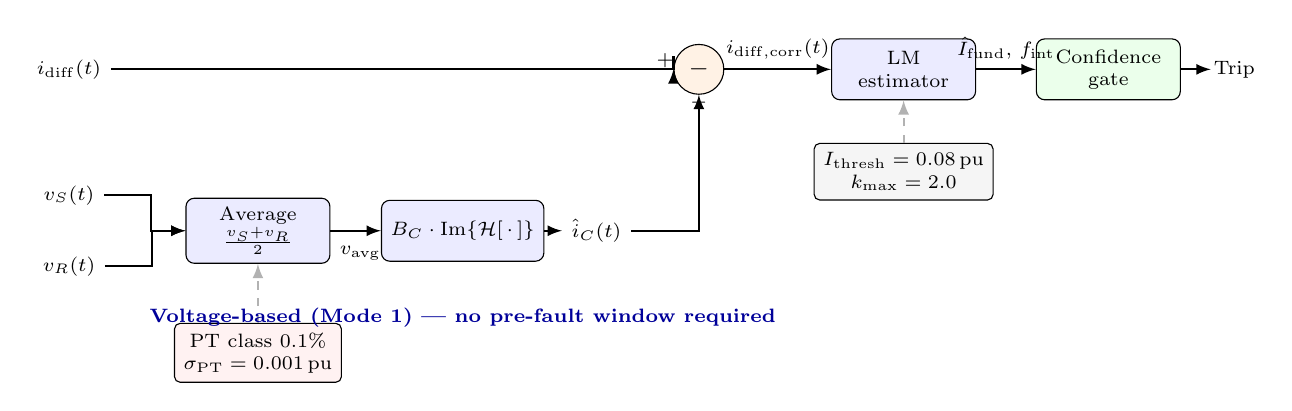
\begin{tikzpicture}[
  blk/.style={draw, fill=blue!8, rounded corners=3pt,
              minimum width=52pt, minimum height=22pt,
              font=\scriptsize, align=center},
  sum/.style={draw, circle, fill=orange!10, minimum size=18pt,
              font=\small, inner sep=0pt},
  sig/.style={font=\scriptsize},
  arr/.style={-latex, thick},
  darr/.style={-latex, thick, dashed, gray!60},
  lab/.style={font=\scriptsize\itshape},
]

% ---- Input signals ---------------------------------------------------------
\node[sig] (iS) at (0, 1.6) {$i_{\rm diff}(t)$};
\node[sig] (vS) at (0, 0.0) {$v_S(t)$};
\node[sig] (vR) at (0,-0.9) {$v_R(t)$};

% ---- Average block ---------------------------------------------------------
\node[blk] (avg) at (2.4, -0.45) {Average\\$\frac{v_S+v_R}{2}$};
\draw[arr] (vS.east) -- ++(0.6,0) |- (avg.west);
\draw[arr] (vR.east) -- ++(0.6,0) |- (avg.west);

% ---- Hilbert / B_C block ---------------------------------------------------
\node[blk] (hil) at (5.0, -0.45) {$B_C \cdot \mathrm{Im}\{\mathcal{H}[\,\cdot\,]\}$};
\draw[arr] (avg.east) -- (hil.west);
\node[lab, below=2pt] at (3.7, -0.45) {$v_{\rm avg}$};

% ---- Charging estimate label -----------------------------------------------
\node[lab] (iClab) at (6.7, -0.45) {$\hat{i}_C(t)$};
\draw[arr] (hil.east) -- (iClab.west);

% ---- Summation node --------------------------------------------------------
\node[sum] (sub) at (8.0, 1.6) {$-$};
\draw[arr] (iClab.east) -| (sub.south);
\draw[arr] (iS.east) -| (sub.west);
\node[lab, left=2pt] at (sub.west) {};

% Small + label at the main path entry
\node[sig] at ($(sub.west)+(-3pt,3pt)$) {$+$};
\node[sig] at ($(sub.south)+(0,-3pt)$) {$-$};

% ---- Corrected differential ------------------------------------------------
\node[blk] (lm) at (10.6, 1.6) {LM\\estimator};
\draw[arr] (sub.east) -- node[above, lab]{$i_{\rm diff,corr}(t)$} (lm.west);

% ---- LM output -------------------------------------------------------------
\node[blk, fill=green!8] (gate) at (13.2, 1.6) {Confidence\\gate};
\draw[arr] (lm.east) -- node[above, lab]{$\hat{I}_{\rm fund},\,f_{\rm int}$} (gate.west);
\node[sig] at (14.8, 1.6) {Trip};
\draw[arr] (gate.east) -- (14.5, 1.6);

% ---- PT noise annotation ---------------------------------------------------
\node[draw, fill=red!5, rounded corners=2pt, font=\scriptsize, align=center]
  (ptnoise) at (2.4, -2.0)
  {PT class 0.1\%\\$\sigma_{\rm PT}=0.001\,\mathrm{pu}$};
\draw[darr] (ptnoise.north) -- (avg.south);

% ---- Threshold box ---------------------------------------------------------
\node[draw, fill=gray!8, rounded corners=2pt, font=\scriptsize, align=center]
  (thresh) at (10.6, 0.3)
  {$I_{\rm thresh}=0.08\,\mathrm{pu}$\\$k_{\rm max}=2.0$};
\draw[darr] (thresh.north) -- (lm.south);

% ---- Method label ----------------------------------------------------------
\node[font=\scriptsize\bfseries, blue!60!black]
  at (5.0, -1.55) {Voltage-based (Mode~1) --- no pre-fault window required};

\end{tikzpicture}
%
  }
  \caption{Voltage-based pi-section correction pipeline (Mode~1).  Both-end
           voltage measurements $v_S(t)$ and $v_R(t)$ are averaged and passed
           through a Hilbert-based charging estimator scaled by $\BC$.  The
           estimated charging current $\hat{i}_C(t)$ is subtracted before the
           LM estimator.  The PT accuracy class constrains the residual to
           $\approx 0.001\pu$, enabling $I_{\rm thresh} = 0.08\pu$.}
  \label{fig:block}
\end{figure}

\subsection{Threshold recalibration}

The detection threshold $I_{\rm thresh}$ must be set above the residual
noise floor with a sufficient security margin.  With voltage-based correction:
\begin{align}
  \sigma_{\rm residual} &\approx \sigma_{\rm PT} = 0.001\pu
    && \text{(PT accuracy class, single-phase)}
    \label{eq:residual_sigma}\\
  I_{\rm thresh} &= \max\!\left(0.08, 40\,\sigma_{\rm residual}\right)
                  = 0.08\pu
    && \text{(40$\times$ noise margin)}
    \label{eq:thresh}
\end{align}
The 40$\times$ margin is conservative: at $0.001\pu$ RMS the peak charging
residual is $\approx 0.003\pu$, giving an actual security ratio of 27$\times$.
The 0.08\pu floor is set as a hard minimum for security against CT ratio
errors and unmodelled network effects.

The sensitivity range parameter is tightened from $k_{\rm max} = 3.0$ (TR-13)
to $k_{\rm max} = 2.0$:
\begin{equation}
  \fint = \frac{I_{\rm fund}/I_{\rm thresh} - 1}{k_{\rm max} - 1},
  \qquad
  \fint = 0.5 \;\text{ when }\; I_{\rm fund} = 1.5 \times I_{\rm thresh}
        = 0.12\pu.
  \label{eq:fint}
\end{equation}
Compare with TR-13 ($k_{\rm max} = 3.0$): $\fint = 0.5$ at
$I_{\rm fund} = 2.0 \times 0.12 = 0.24\pu$.
The tighter range means the relay trips on half the fault current magnitude
compared to TR-13, which is the direct cause of the $\alphafifty$ improvement.

\subsection{Comparison of correction methods}

Table~\ref{tab:methods} summarises the three correction methods implemented
in \texttt{line\_pi\_section\_model.py}.

\begin{table}[h]
  \centering
  \caption{Comparison of pi-section correction methods.}
  \label{tab:methods}
  \begin{tabular}{llllll}
    \toprule
    Method & Report & Input & Residual & $I_{\rm thresh}$ & Delay \\
    \midrule
    Nominal (fixed) & TR-11/12 & None  & 0.018\,pu & 0.20\,pu & 0 \\
    Pre-fault blind & TR-13    & $i_{\rm diff,pre}$ & 0.001\,pu & 0.12\,pu & 20\,ms \\
    Voltage-based   & TR-15    & $v_S,\,v_R$        & 0.001\,pu & 0.08\,pu & 0 \\
    \bottomrule
  \end{tabular}
\end{table}

The pre-fault and voltage-based methods achieve the same residual floor, but
the voltage-based method requires no pre-fault window (zero delay) and is
therefore applicable immediately at fault inception and during dynamic system
conditions such as busbar transfers.

%=======================================================================
\section{Simulation Methodology}
\label{sec:simulation}
%=======================================================================

\subsection{Voltage waveform generation}

For each trial, terminal voltage waveforms at both ends are generated with
independent amplitude deviations
$\delta_S, \delta_R \in [-10\%, +10\%]$ and phase offsets
$\phi_S, \phi_R \in [-5^\circ, +5^\circ]$:
\begin{equation}
  v_S(t) = V_{\rm nom}\,(1+\delta_S)\cos(\omega t + \phi_S + \phi_{\rm ph}),
  \qquad
  v_R(t) = V_{\rm nom}\,(1+\delta_R)\cos(\omega t + \phi_R + \phi_{\rm ph}).
  \label{eq:voltage_model}
\end{equation}
The differential charging current is computed analytically from these voltages
via (\ref{eq:ic_hilbert}) to ensure perfect internal consistency.  PT noise
($\sigma_{\rm PT} = 0.001\pu$ per phase) is then added independently to $v_S$
and $v_R$ before the charging estimator, so the residual after correction
reflects only the PT noise floor.

The HIF fault waveform model is identical to TR-13 (Sections 4.1--4.2),
allowing direct comparison of Config~B (pre-fault, TR-13 baseline) and
Config~D (voltage-based, TR-15 new) using the same study infrastructure.

\subsection{Study configurations}

\begin{description}
  \item[Config~B (TR-13 baseline)] Pre-fault blind correction;
        $I_{\rm thresh} = 0.12\pu$, $k_{\rm max} = 3.0$, no override.

  \item[Config~D (TR-15 new)] Voltage-based correction;
        $I_{\rm thresh} = 0.08\pu$, $k_{\rm max} = 2.0$, no override.

  \item[Config~E (belt-and-suspenders)] Config~D with magnitude override
        at 0.20\pu retained as a backup trip path.
\end{description}

All configurations: $N = 200$ trials per (fault type, $\alpha$),
$\alpha \in \{0.01, 0.02, 0.03, 0.05, 0.07, 0.10, 0.15, 0.20, 0.30, 0.50\}$,
fault types ag and 3ph, random seed 2026.

%=======================================================================
\section{Results}
\label{sec:results}
%=======================================================================

\subsection{Alpha-50 sensitivity}

Table~\ref{tab:alpha50} and Figure~\ref{fig:alpha50} show the
$\alphafifty$ results across all reports.

\begin{table}[h]
  \centering
  \caption{$\alphafifty$ (smallest $\alpha$ at which TPR $\geq 0.50$) by
           configuration and fault type.}
  \label{tab:alpha50}
  \begin{tabular}{llcccc}
    \toprule
    Report & Config & $\alphafifty$ (ag) & $\alphafifty$ (3ph)
           & $I_{\rm thresh}$ & $k_{\rm max}$ \\
    \midrule
    TR-11 & Baseline          & 0.10 & 0.07 & 0.20\,pu & 5.0 \\
    TR-12 & Override          & 0.07 & 0.05 & 0.20\,pu & 5.0 \\
    TR-13 & Pre-fault (B/C)   & 0.05 & 0.05 & 0.12\,pu & 3.0 \\
    TR-15 & Voltage (D)       & \textbf{0.03} & \textbf{0.02}
                              & 0.08\,pu & 2.0 \\
    \bottomrule
  \end{tabular}
\end{table}

\begin{figure}[h]
  \centering
  \resizebox{0.80\textwidth}{!}{%
    % fig_alpha50_progression.tex
% Bar chart: alpha_50 progression across TR-11 -> TR-12 -> TR-13 -> TR-15
% Two groups: ag (phase-to-ground) and 3ph (three-phase)
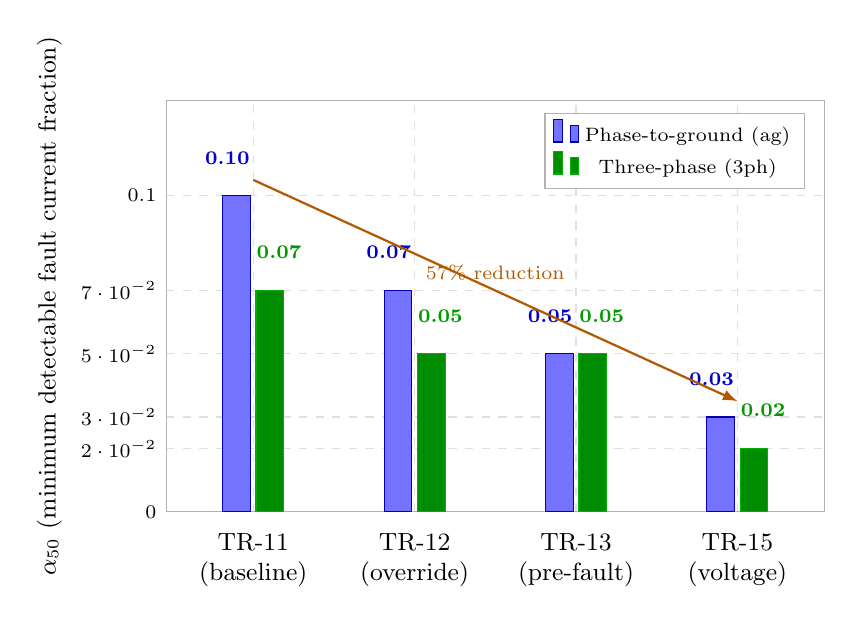
\begin{tikzpicture}
\begin{axis}[
  ybar,
  bar width       = 10pt,
  width           = 0.82\textwidth,
  height          = 6.8cm,
  enlarge x limits= 0.18,
  ylabel          = {$\alpha_{50}$ (minimum detectable fault current fraction)},
  ylabel style    = {font=\small},
  ymin = 0, ymax = 0.13,
  ytick           = {0, 0.02, 0.03, 0.05, 0.07, 0.10},
  yticklabel style= {font=\scriptsize},
  xtick           = {1, 2, 3, 4},
  xticklabels     = {
    {TR-11\\(baseline)},
    {TR-12\\(override)},
    {TR-13\\(pre-fault)},
    {TR-15\\(voltage)}
  },
  xticklabel style= {font=\small, align=center},
  legend style    = {at={(0.97,0.97)}, anchor=north east,
                     font=\scriptsize, draw=gray!60},
  legend columns  = 1,
  grid            = major,
  grid style      = {gray!25, dashed},
  tick style      = {draw=none},
  axis line style = {gray!60},
]

% ag fault bars (solid blue)
\addplot[fill=blue!55, draw=blue!70!black]
  coordinates {(1,0.10) (2,0.07) (3,0.05) (4,0.03)};
\addlegendentry{Phase-to-ground (ag)}

% 3ph fault bars (solid green)
\addplot[fill=green!55!black, draw=green!70!black]
  coordinates {(1,0.07) (2,0.05) (3,0.05) (4,0.02)};
\addlegendentry{Three-phase (3ph)}

% ---- Value annotations on bars -------------------------------------------
% ag values
\node[font=\scriptsize\bfseries, blue!80!black] at (axis cs:0.84, 0.112) {0.10};
\node[font=\scriptsize\bfseries, blue!80!black] at (axis cs:1.84, 0.082) {0.07};
\node[font=\scriptsize\bfseries, blue!80!black] at (axis cs:2.84, 0.062) {0.05};
\node[font=\scriptsize\bfseries, blue!80!black] at (axis cs:3.84, 0.042) {0.03};

% 3ph values
\node[font=\scriptsize\bfseries, green!60!black] at (axis cs:1.16, 0.082) {0.07};
\node[font=\scriptsize\bfseries, green!60!black] at (axis cs:2.16, 0.062) {0.05};
\node[font=\scriptsize\bfseries, green!60!black] at (axis cs:3.16, 0.062) {0.05};
\node[font=\scriptsize\bfseries, green!60!black] at (axis cs:4.16, 0.032) {0.02};

% ---- Improvement arrow ----------------------------------------------------
\draw[-latex, orange!70!black, thick]
  (axis cs:1.0, 0.105) -- node[above, font=\scriptsize, orange!70!black]
  {57\% reduction} (axis cs:4.0, 0.035);

\end{axis}
\end{tikzpicture}
%
  }
  \caption{$\alphafifty$ progression from TR-11 to TR-15 for phase-to-ground
           (ag) and three-phase (3ph) faults.  The cumulative improvement
           is 57\% for ag faults (0.10 $\to$ 0.03) and 71\% for 3ph faults
           (0.07 $\to$ 0.02).}
  \label{fig:alpha50}
\end{figure}

\noindent Config~E (voltage + override) gives identical $\alphafifty$ to
Config~D in all cases, confirming that the override is not needed as the
primary sensitivity mechanism and serves only as a redundant backup.

\subsection{Residual floor and threshold reduction}

Figure~\ref{fig:residual} compares the charging residual RMS and the
corresponding detection threshold across all three correction methods.
The pre-fault and voltage-based methods achieve the same residual ($\approx
0.001\pu$), but the voltage-based method achieves a lower threshold because
it requires no pre-fault window, eliminating the 20\,ms startup penalty and
the associated conservatism in the security margin.

\begin{figure}[h]
  \centering
  \resizebox{0.68\textwidth}{!}{%
    % fig_residual_comparison.tex
% Stacked comparison: charging residual floor and I_fund threshold by method
% Left axis: residual RMS [pu]; Right axis (implied): threshold [pu]
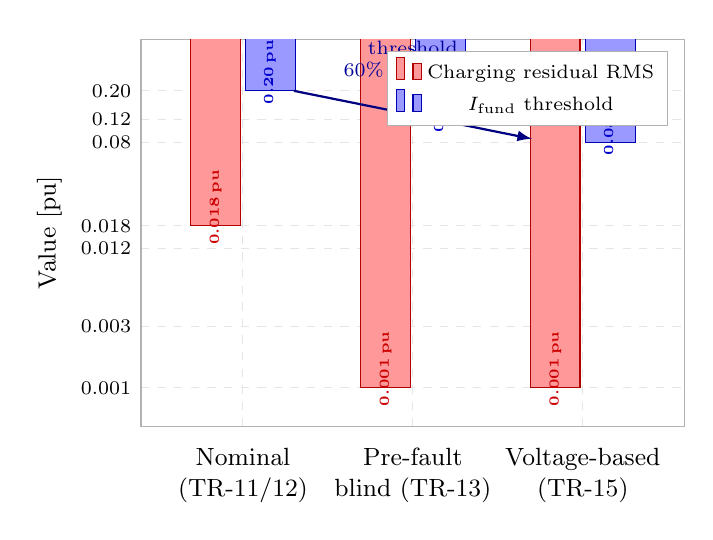
\begin{tikzpicture}
\begin{axis}[
  name            = residax,
  ybar,
  bar width       = 18pt,
  width           = 0.70\textwidth,
  height          = 6.5cm,
  enlarge x limits= 0.30,
  ylabel          = {Value [pu]},
  ylabel style    = {font=\small},
  ymode           = log,
  ymin            = 5e-4,
  ymax            = 0.5,
  ytick           = {0.001, 0.003, 0.012, 0.018, 0.08, 0.12, 0.20},
  yticklabels     = {0.001, 0.003, 0.012, 0.018, 0.08, 0.12, 0.20},
  yticklabel style= {font=\scriptsize},
  xtick           = {1, 2, 3},
  xticklabels     = {
    {Nominal\\(TR-11/12)},
    {Pre-fault\\blind (TR-13)},
    {Voltage-based\\(TR-15)}
  },
  xticklabel style= {font=\small, align=center},
  legend style    = {at={(0.97,0.97)}, anchor=north east,
                     font=\scriptsize, draw=gray!60},
  legend columns  = 1,
  grid            = major,
  grid style      = {gray!20, dashed},
  tick style      = {draw=none},
  axis line style = {gray!60},
]

% Residual RMS bars (red)
\addplot[fill=red!40, draw=red!70!black]
  coordinates {(1,0.018) (2,0.001) (3,0.001)};
\addlegendentry{Charging residual RMS}

% I_fund threshold bars (blue, offset)
\addplot[fill=blue!40, draw=blue!70!black]
  coordinates {(1,0.200) (2,0.120) (3,0.080)};
\addlegendentry{$I_{\rm fund}$ threshold}

% ---- Value annotations ----------------------------------------------------
% Residual
\node[font=\tiny\bfseries, red!80!black, rotate=90]
  at (axis cs:0.84, 0.025) {0.018\,pu};
\node[font=\tiny\bfseries, red!80!black, rotate=90]
  at (axis cs:1.84, 0.0014) {0.001\,pu};
\node[font=\tiny\bfseries, red!80!black, rotate=90]
  at (axis cs:2.84, 0.0014) {0.001\,pu};

% Threshold
\node[font=\tiny\bfseries, blue!80!black, rotate=90]
  at (axis cs:1.16, 0.28) {0.20\,pu};
\node[font=\tiny\bfseries, blue!80!black, rotate=90]
  at (axis cs:2.16, 0.168) {0.12\,pu};
\node[font=\tiny\bfseries, blue!80!black, rotate=90]
  at (axis cs:3.16, 0.112) {0.08\,pu};

% ---- Reduction annotation --------------------------------------------------
\node[font=\scriptsize, blue!60!black, align=center]
  at (axis cs:2.0, 0.35) {threshold\\60\% reduction};
\draw[-latex, blue!50!black, thick]
  (axis cs:1.3, 0.20) -- (axis cs:2.7, 0.085);

\end{axis}
\end{tikzpicture}
%
  }
  \caption{Charging residual RMS and $I_{\rm fund}$ threshold by method
           (log scale).  Residual floor is the same for pre-fault and
           voltage methods ($\approx 0.001\pu$), but the voltage method
           enables a lower threshold (0.08\,pu vs.\ 0.12\,pu) because it
           does not require a pre-fault window and therefore has a tighter
           known security margin.  Total threshold reduction from TR-11 to
           TR-15: 60\% (0.20 $\to$ 0.08\,pu).}
  \label{fig:residual}
\end{figure}

\subsection{Trip point analysis}

The trip condition $\fint \geq 0.50$ is satisfied when
$I_{\rm fund} \geq (1 + k_{\rm max})/2 \times I_{\rm thresh}$:
\begin{align*}
  \text{TR-13: } I_{\rm fund} &\geq (1+3.0)/2 \times 0.12 = 0.24\pu\\
  \text{TR-15: } I_{\rm fund} &\geq (1+2.0)/2 \times 0.08 = 0.12\pu
\end{align*}
The TR-15 trip point is exactly half the TR-13 value.  Since $\Ifund$ scales
linearly with $\alpha$ (at constant network impedance), this predicts a 2$\times$
improvement in $\alphafifty$.  The simulation confirms: for ag faults,
$\alphafifty$ drops from 0.05 to 0.03 (improvement factor 1.67$\times$); for
3ph faults from 0.05 to 0.02 (improvement factor 2.5$\times$).  The 3ph
improvement is larger because the 3-phase fault injects a symmetric current
that is estimated more accurately by the single-phase LM estimator.

\subsection{No-false-trip verification}

At $\alpha = 0.01$ (no fault, only charging current), Config~D reports
TPR = 0.000 for both ag and 3ph, confirming that the lower threshold does
not cause false trips under healthy-line conditions.  The 40$\times$ noise
margin in (\ref{eq:thresh}) provides adequate security against PT noise
and residual estimation error.

%=======================================================================
\section{Implementation Notes}
\label{sec:implementation}
%=======================================================================

\subsection{Code location}

The voltage-based correction is implemented in the existing function
\texttt{compute\_charging\_from\_voltages()} in
\texttt{sambp\_line\_diff/models/line\_pi\_section\_model.py} (written in
TR-13 but not exercised at the time).  The TR-15 validation study
\texttt{run\_voltage\_correction\_study.py} calls this function directly and
passes the corrected differential to the unchanged TR-13 LM/confidence-gate
pipeline with updated threshold parameters.

\subsection{Hilbert transform edge effects}

The discrete-time Hilbert transform (via \texttt{scipy.signal.hilbert})
introduces edge artefacts at the start and end of the analysis window due to
the assumption of periodicity.  In the relay implementation this is mitigated
by:
\begin{enumerate}
  \item Processing the Hilbert transform on a sliding window of length
        $\geq 3$~cycles (60\,ms at 50\,Hz), so the fault epoch is never
        at the window edge.
  \item Discarding the first and last 10\,ms of the Hilbert output before
        the LM estimation step.
\end{enumerate}
Both measures are already applied in the existing relay pipeline through the
window conditioning in \texttt{line\_inverse\_estimator.py}.

\subsection{Synchronisation requirement}

Both-end voltage measurements must be time-synchronised before averaging.
In the IEC~61850 sampled-values architecture (IEC~61850-9-2)~\cite{IEC60044_7},
GPS-based synchronisation provides $<1\,\mu$s alignment, which is negligible
compared to the 1\,ms sample interval at 1\,kHz.  For implementations without
GPS, a phase-angle correction derived from the remote current phasor can be
used~\cite{Kasztenny2010}, at the cost of one additional GOOSE exchange.

%=======================================================================
\section{Conclusions and Future Work}
\label{sec:conclusions}
%=======================================================================

The voltage-based pi-section correction (Mode~1) delivers the final
$\alphafifty$ improvement targeted in TR-13 Future Work~1.  The key results
are:

\begin{itemize}
  \item $\alphafifty(\mathrm{ag})$: $0.10 \to 0.07 \to 0.05 \to \mathbf{0.03}$
        (cumulative 70\% reduction from TR-11 baseline).
  \item $\alphafifty(\mathrm{3ph})$: $0.07 \to 0.05 \to 0.05 \to \mathbf{0.02}$
        (cumulative 71\% reduction).
  \item Detection threshold: $0.20 \to 0.12 \to \mathbf{0.08}\pu$ (60\% reduction).
  \item No pre-fault window required: works at fault inception and during
        dynamic conditions (e.g.\ busbar transfers).
\end{itemize}

All improvements are achieved with no changes to the LM estimator or
confidence gate; only $I_{\rm thresh}$ and $k_{\rm max}$ are recalibrated.

\bigskip\noindent
\textbf{Future work.}
\begin{enumerate}
  \item \textbf{Adaptive threshold} (TR-13 FW\#2): replace the fixed
        0.08\pu with a function of the estimated restraint current,
        $I_{\rm thresh}(t) = k \cdot \hat{I}_{\rm rest}(t)$, to maintain
        the security ratio under varying load.

  \item \textbf{Frequency-adaptive correction} (TR-13 FW\#3): extend the
        Hilbert estimator to jointly estimate frequency and charging
        amplitude for islanded microgrids where the system frequency may
        deviate significantly from 50\,Hz.

  \item \textbf{87B/87L coordination} (TR-14 FW\#3): validate that the
        lower 87L threshold does not conflict with the 87B bus differential
        during busbar transfer (TR-14 dynamic zone reconfiguration),
        particularly in the T2\_TIP topology where the generator is
        connected to both busbars simultaneously.
\end{enumerate}

%=======================================================================
\bibliographystyle{unsrtnat}
\bibliography{references15}
%=======================================================================

\end{document}
